\newpage
\section{Experiment Results}
\label{sec:results}

\subsection{Experimental Setup}
\label{subsec:results-setup}

All experiments were conducted on a Windows workstation using the local Java-Python co-simulation pipeline described in \Secref{sec:simulation}. The software stack includes OpenJDK 25.0.1 LTS, Python 3.9.13, Maven 3.9.12, and PyTorch 2.8.0. The main hardware configuration is listed in \Tabref{tab:hardware-config}.

\begin{table}[htbp]
    \centering
    \begin{tabular}{p{0.34\linewidth}p{0.46\linewidth}}
        \hline
        \textbf{Component} & \textbf{Configuration} \\
        \hline
        CPU & 11th Gen Intel Core i7-11800H @ 2.30 GHz \\
        GPU & NVIDIA RTX A2000 Laptop GPU \\
        System memory & 31.67 GB RAM \\
        Operating system & Windows \\
        Java runtime & OpenJDK 25.0.1 LTS \\
        Python runtime & Python 3.9.13 \\
        Build tool & Maven 3.9.12 \\
        Deep learning library & PyTorch 2.8.0 \\
        Plotting library & matplotlib 3.9.2 \\
        \hline
    \end{tabular}
    \caption{Hardware and software configuration used for training and evaluation.}
    \label{tab:hardware-config}
\end{table}

The evaluation focuses on the following metrics.
\begin{itemize}
    \item \textbf{Task success rate:} percentage of tasks that finish within their latency constraints.
    \item \textbf{Average total time:} end-to-end delay including waiting, execution, and transfer stages.
    \item \textbf{Energy consumption:} average transmission-related energy reported by the simulator.
    \item \textbf{Destination distribution:} percentage of decisions assigned to local, edge, and cloud destinations.
    \item \textbf{PRB usage:} empirical selection frequency of PRB bins chosen by the policy.
\end{itemize}

Two types of artifacts are currently available in the workspace. First, a complete three-seed MAPPO evaluation export provides structured JSON summaries for quantitative analysis. Second, representative heuristic baselines are preserved as dashboard images rather than CSV tables. Therefore, this section combines exact MAPPO measurements with qualitative cross-algorithm comparisons from the available dashboards.

\subsection{Training Performance}
\label{subsec:training-performance}

\Figref{fig:training-success-latency} summarizes the training trajectories available in the workspace. The MAPPO curve is based on a 40-episode run, while the PPO comparison curve is shorter and is used only as an early-stage reference. Both algorithms improve rapidly during the first ten episodes, but MAPPO continues to stabilize near perfect task success while pushing the latency proxy downward.

\begin{figure}[htbp]
    \centering
    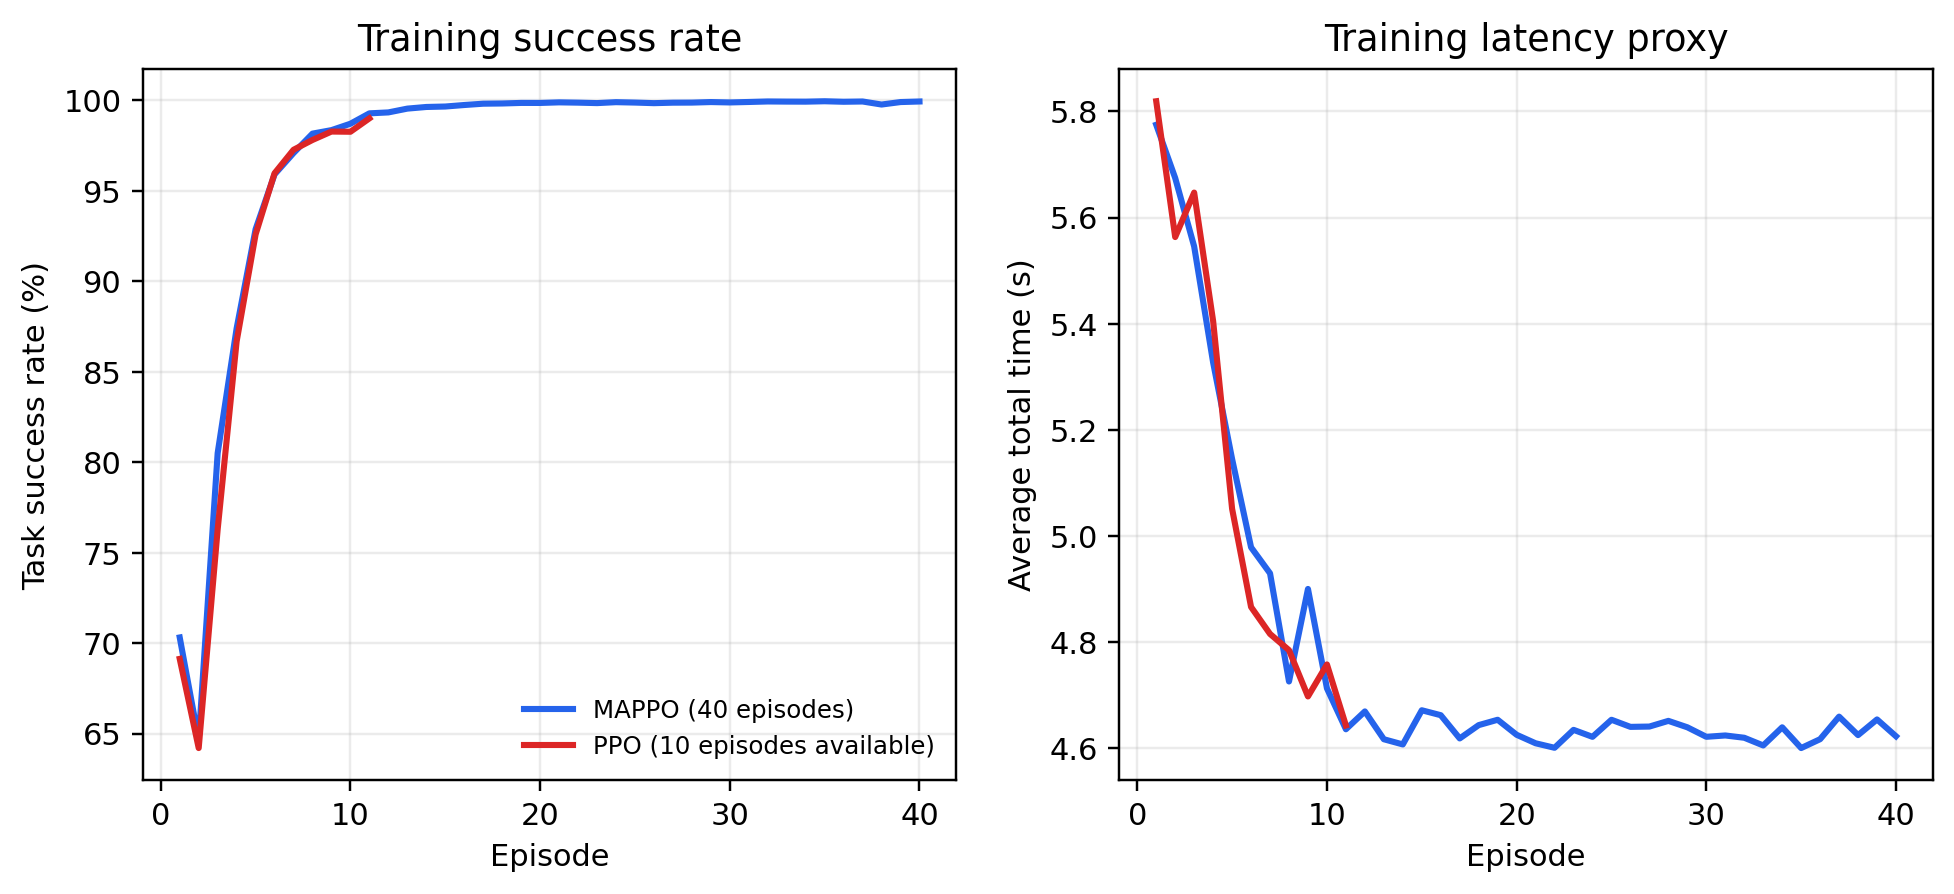
\includegraphics[width=0.92\textwidth]{figures/training_success_latency.png}
    \caption{Training curves for MAPPO and the available PPO baseline artifact.}
    \label{fig:training-success-latency}
\end{figure}

The MAPPO training curve increases from roughly \(70\%\) task success in the first episode to above \(99.5\%\) after about twelve episodes, and then remains essentially saturated for the rest of the run. In parallel, the average total-time proxy drops from about \(5.8\,\mathrm{s}\) to approximately \(4.6\,\mathrm{s}\). This pattern suggests that the policy first learns to avoid catastrophic failures and then fine-tunes latency-sensitive destination and PRB decisions.

The PPO baseline follows a similar initial trend, which indicates that the environment is learnable with on-policy methods. However, the available PPO export is shorter and less complete than the MAPPO artifact, so the later-stage comparison is best interpreted as suggestive rather than definitive.

\subsection{Task Success Rate Comparison}
\label{subsec:task-success-comparison}

The structured three-seed MAPPO evaluation is shown in \Figref{fig:mappo-eval-overview}. The measured task success rates are \(99.9346\%\), \(99.9346\%\), and \(99.9510\%\) for random seeds 9001, 9002, and 9003, respectively, corresponding to an average of \(99.9401\%\). This is an extremely small variance for a stochastic simulator and indicates that the learned policy is highly stable.

\begin{figure}[htbp]
    \centering
    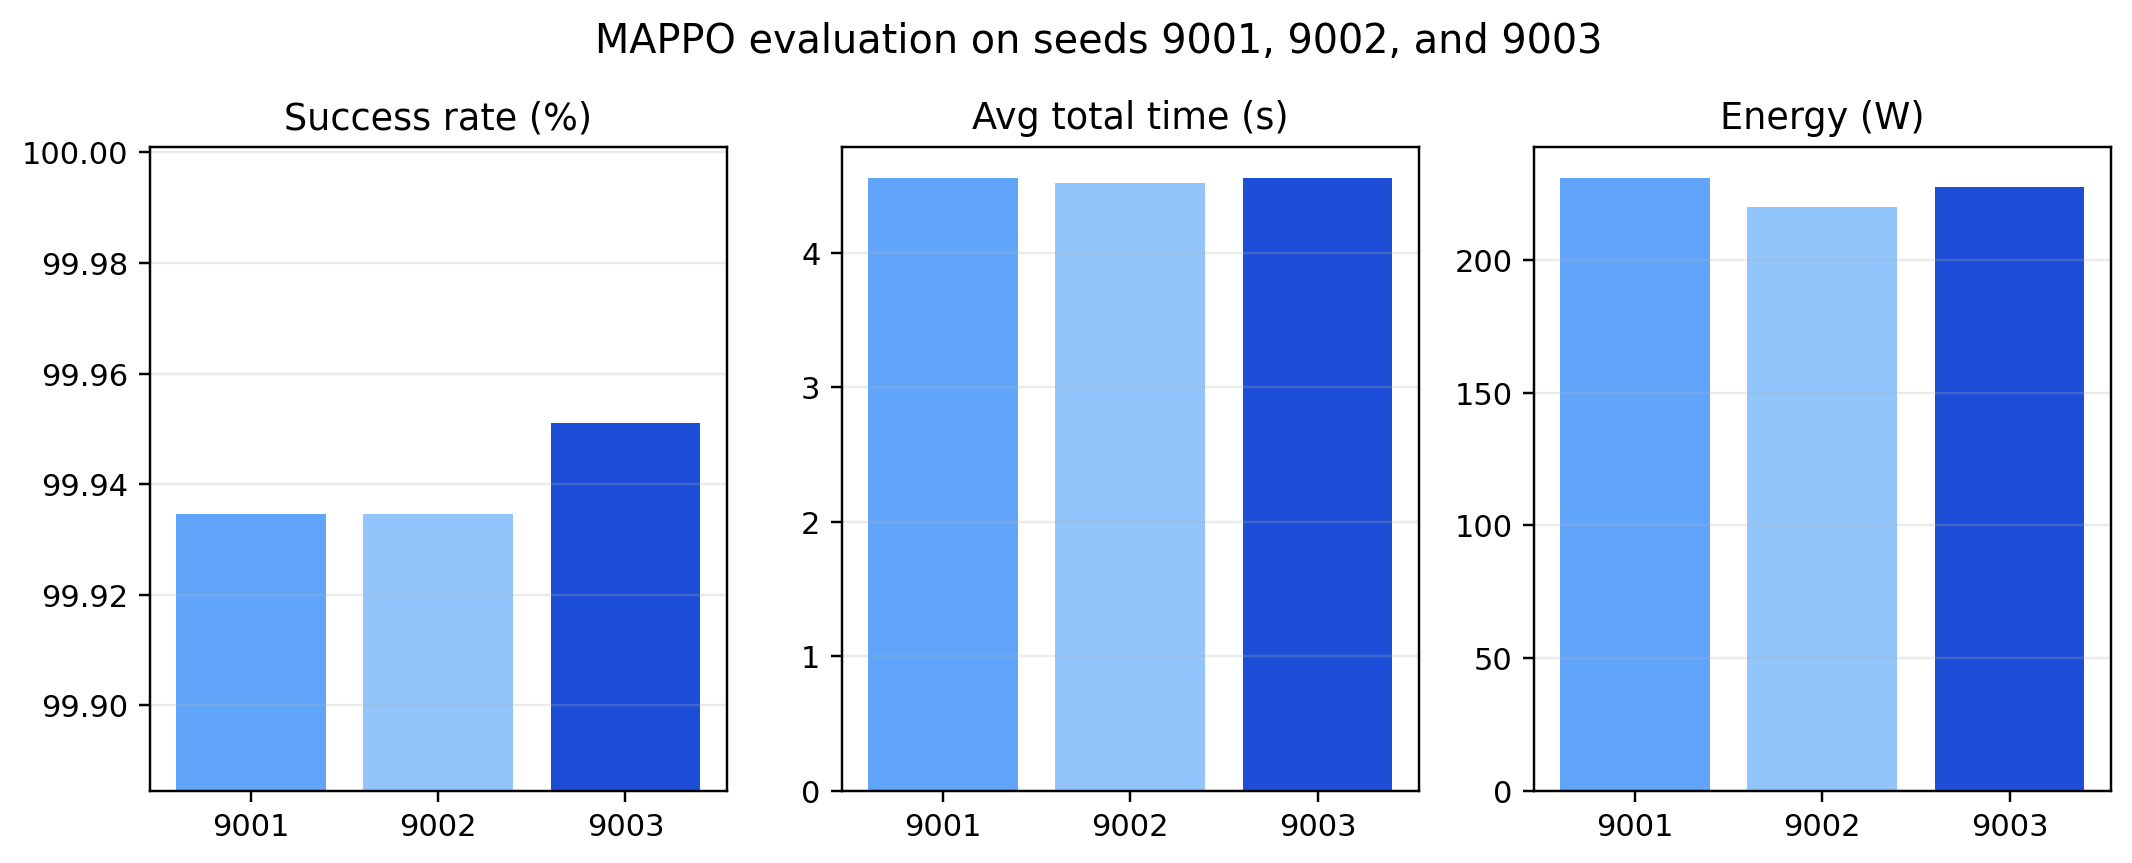
\includegraphics[width=0.92\textwidth]{figures/mappo_eval_overview.png}
    \caption{MAPPO evaluation metrics over three independent random seeds.}
    \label{fig:mappo-eval-overview}
\end{figure}

To place MAPPO in context, \Figref{fig:baseline-dashboards} compares representative dashboard outputs for LOCAL, TRADE\_OFF, and MAPPO. These are visual summaries rather than structured CSV exports, so the baseline readings should be interpreted qualitatively. Even so, the difference is clear: LOCAL degrades into the mid-\(90\%\) success-rate region, TRADE\_OFF drops far lower because of accumulated failures, while MAPPO maintains a near-flat success curve at almost \(100\%\).

\begin{figure}[htbp]
    \centering
    \begin{minipage}{0.32\textwidth}
        \centering
        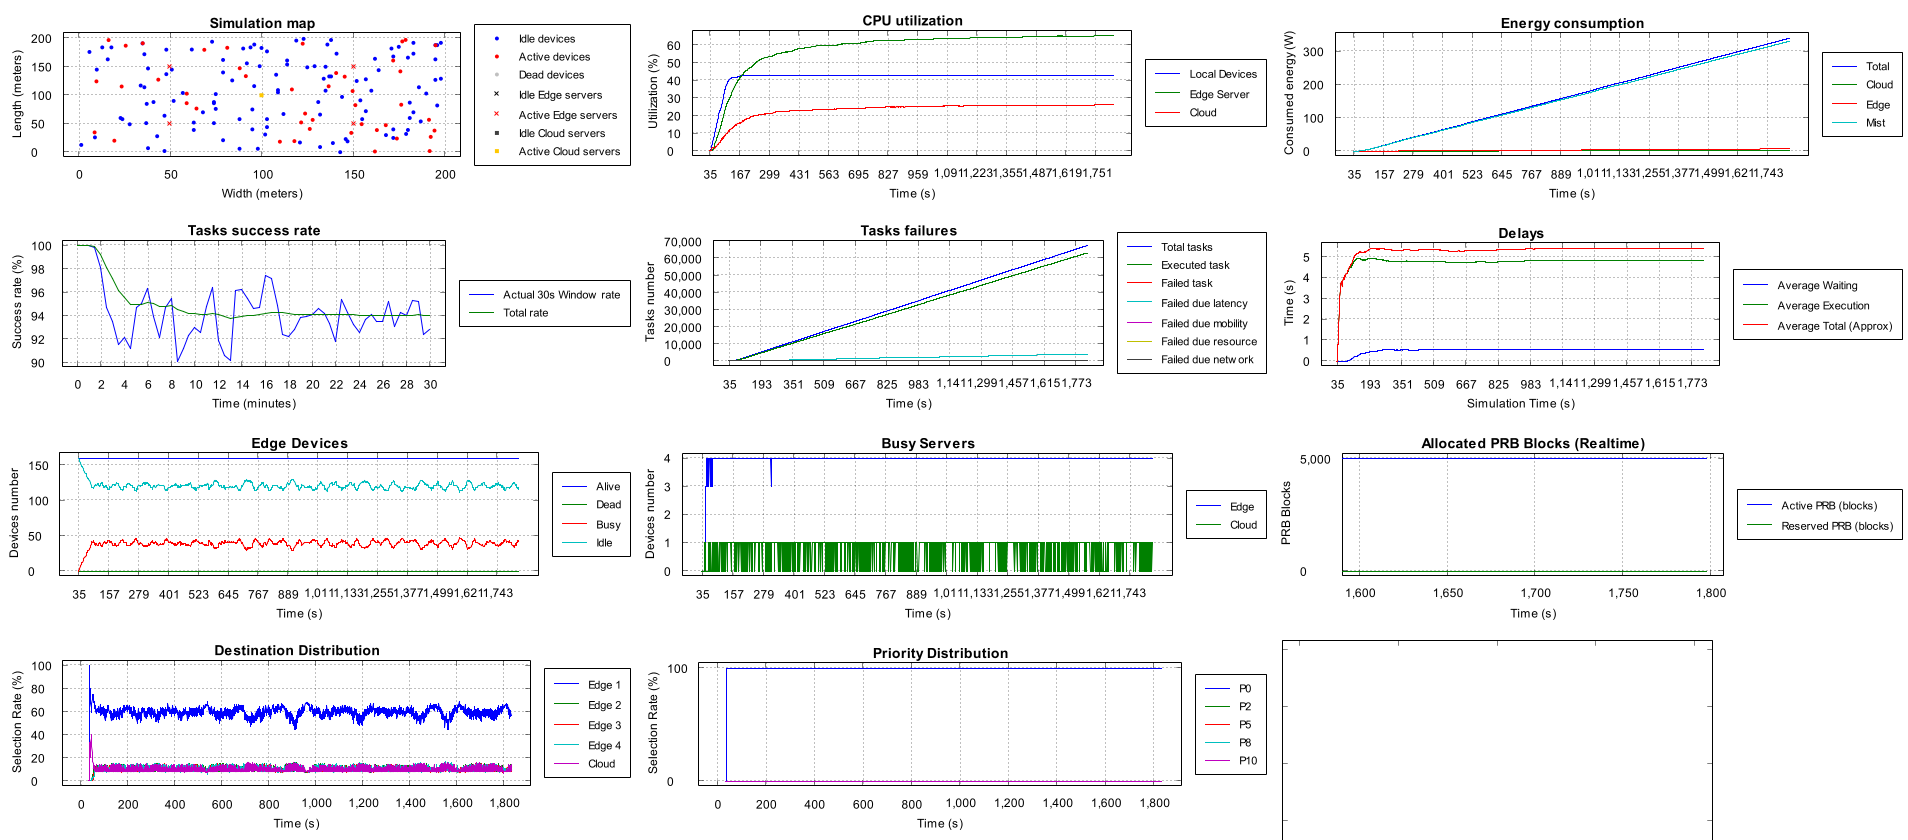
\includegraphics[width=\textwidth]{figures/dashboard_local.png}
    \end{minipage}
    \hfill
    \begin{minipage}{0.32\textwidth}
        \centering
        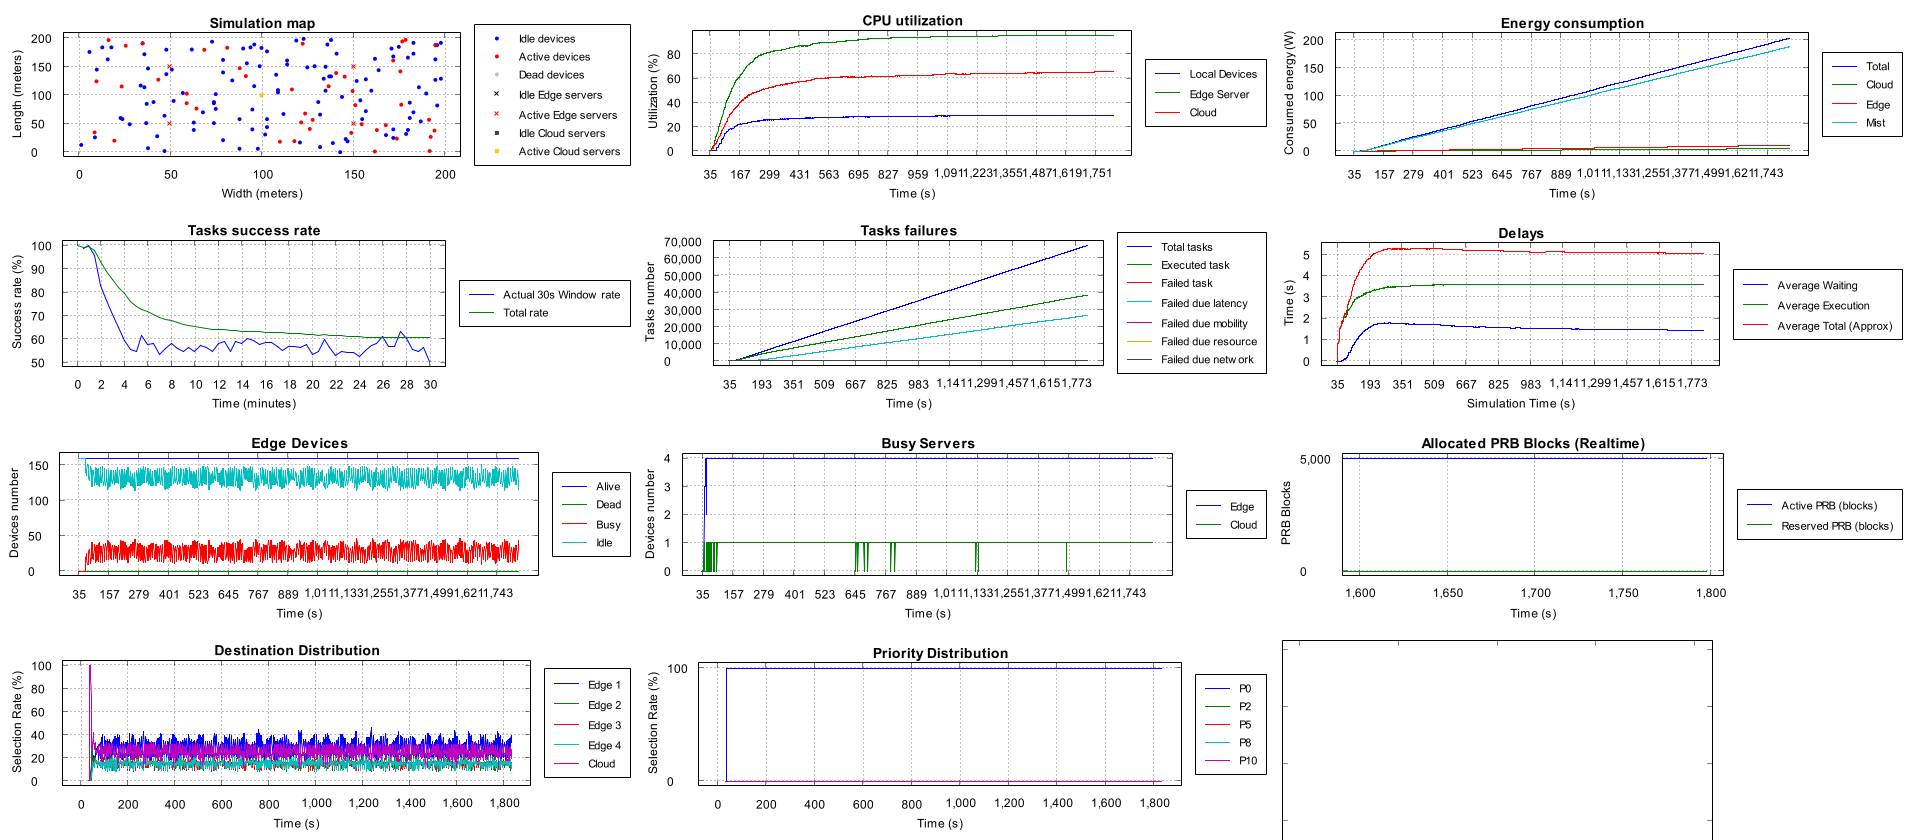
\includegraphics[width=\textwidth]{figures/dashboard_tradeoff.png}
    \end{minipage}
    \hfill
    \begin{minipage}{0.32\textwidth}
        \centering
        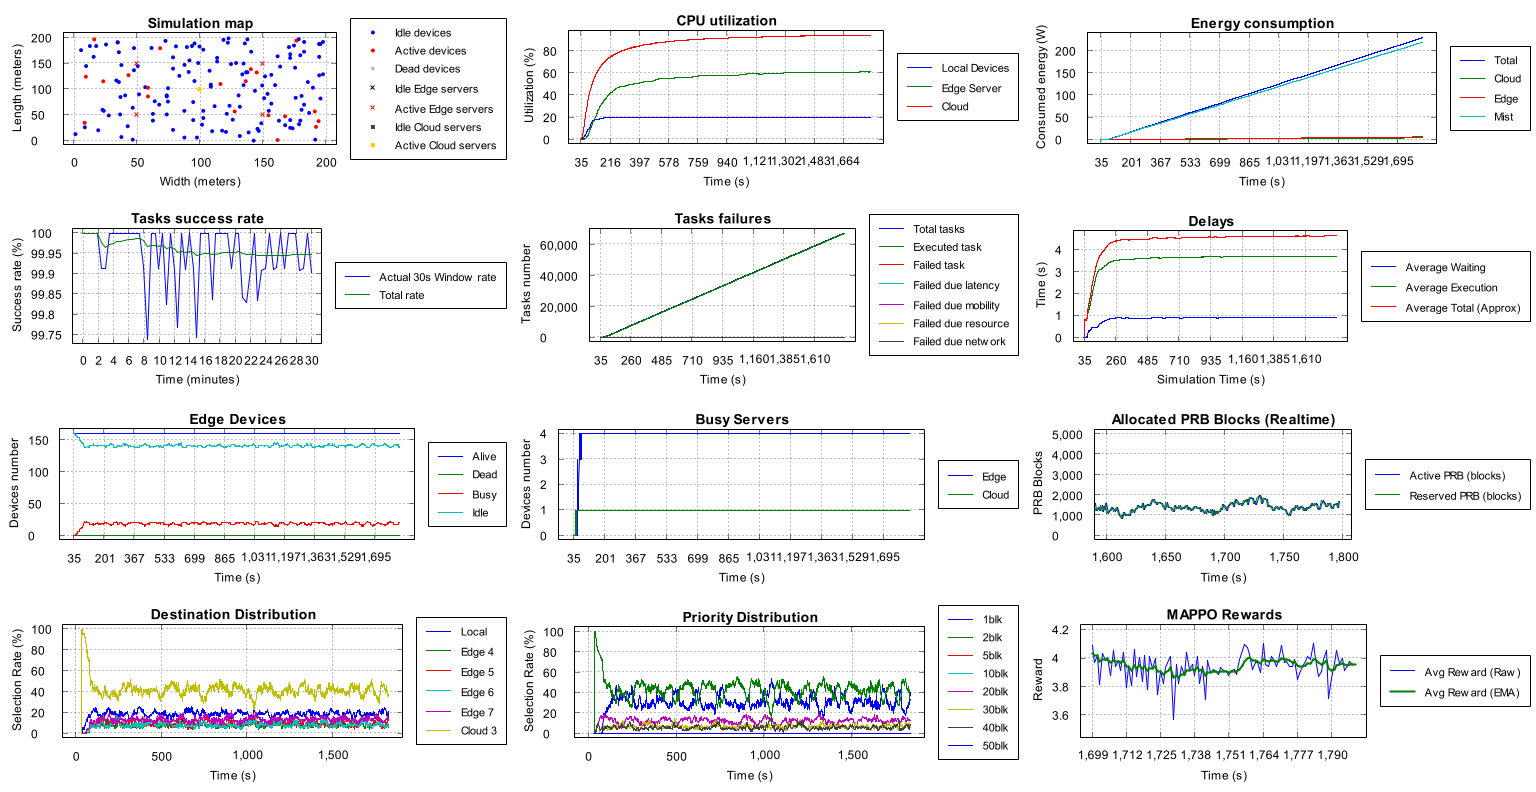
\includegraphics[width=\textwidth]{figures/dashboard_mappo.png}
    \end{minipage}
    \caption{Representative dashboards for LOCAL, TRADE\_OFF, and MAPPO. The baseline comparison is qualitative because the preserved artifacts are dashboard images rather than CSV summaries.}
    \label{fig:baseline-dashboards}
\end{figure}

\subsection{Latency Analysis}
\label{subsec:latency-analysis}

Across seeds 9001, 9002, and 9003, MAPPO achieves an average total time of \(4.5434\,\mathrm{s}\). The corresponding average waiting time is \(0.9200\,\mathrm{s}\), while the average execution delay is \(3.6233\,\mathrm{s}\). These numbers indicate that most of the end-to-end delay comes from execution rather than queueing, which is consistent with the substantial fraction of tasks intentionally sent to the higher-capacity cloud tier.

The dashboard comparison also suggests that MAPPO reduces delay relative to the heuristic baselines shown in \Figref{fig:baseline-dashboards}. LOCAL stabilizes at a visibly higher total-time level of roughly \(5.3\,\mathrm{s}\), while TRADE\_OFF remains near \(5.0\,\mathrm{s}\). In contrast, MAPPO stabilizes close to \(4.5\,\mathrm{s}\), showing that the learned policy finds a better balance between short-range local processing and higher-capacity remote execution.

\subsection{Energy Consumption Analysis}
\label{subsec:energy-analysis}

The mean MAPPO energy consumption over the three evaluation seeds is \(226.0822\) in the simulator's reported energy unit. The individual runs range from \(219.7854\) to \(231.0655\), which is a moderate spread compared with the much larger improvement in success rate. This indicates that the policy is not simply minimizing energy at the expense of deadlines; instead, it trades some extra energy for more reliable completion.

The qualitative dashboards support this interpretation. LOCAL accumulates noticeably higher total energy than MAPPO because many tasks remain on weaker or congested resources for longer periods. TRADE\_OFF appears slightly lower-energy than MAPPO, but this comes with a substantial collapse in task success rate. MAPPO therefore occupies a more useful operating point on the energy-performance frontier.

\subsection{Destination Distribution Analysis}
\label{subsec:destination-analysis}

\Figref{fig:mappo-destination-distribution} shows the destination selection distribution averaged over the three MAPPO evaluation seeds. The learned policy chooses local execution for \(19.42\%\) of decisions, distributes \(40.99\%\) of tasks across the four edge data centers, and sends \(39.60\%\) of tasks to the cloud.

\begin{figure}[htbp]
    \centering
    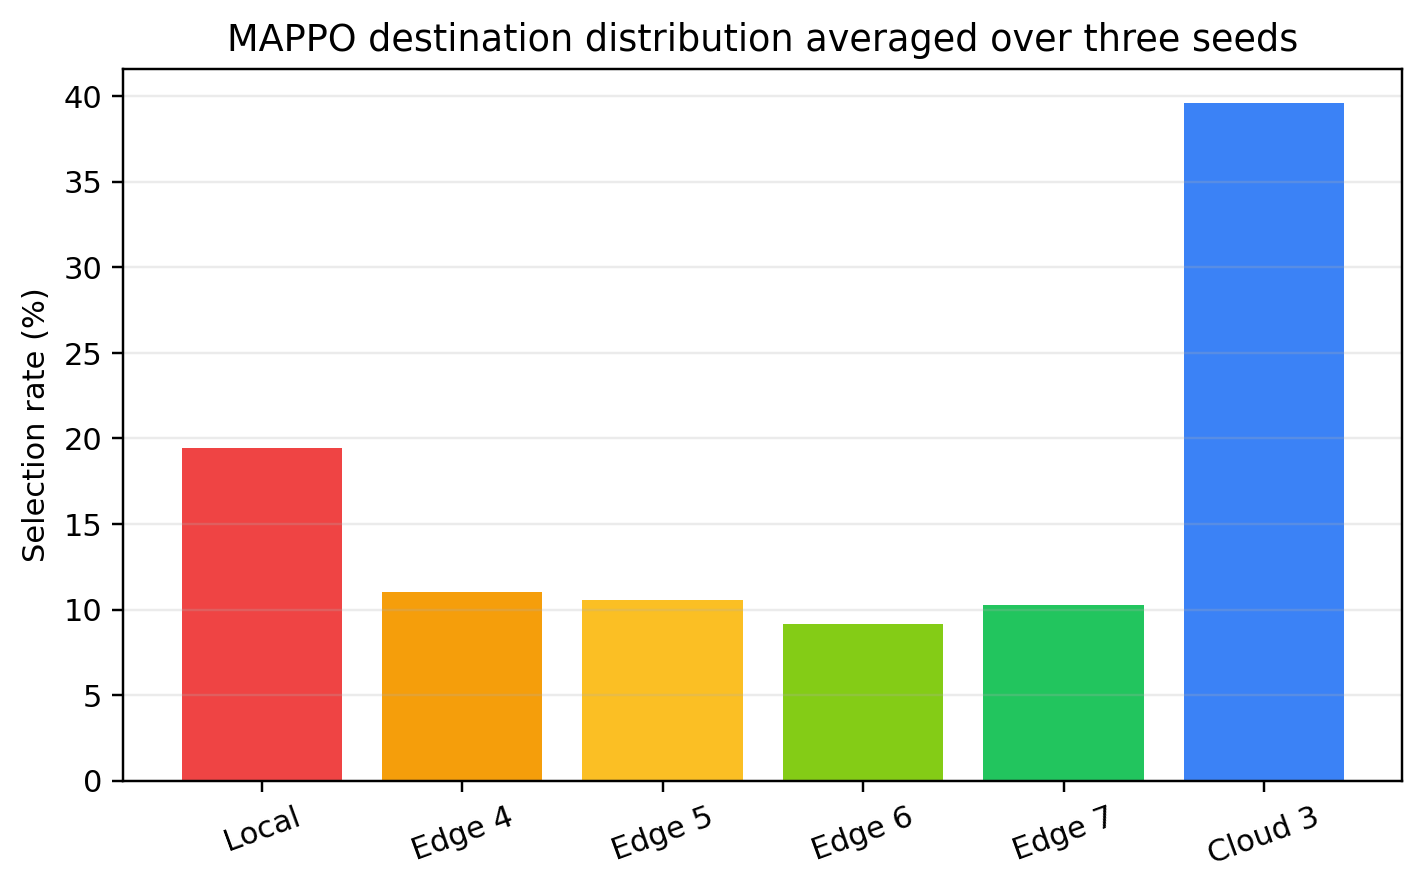
\includegraphics[width=0.88\textwidth]{figures/mappo_destination_distribution.png}
    \caption{MAPPO destination selection distribution averaged over three seeds.}
    \label{fig:mappo-destination-distribution}
\end{figure}

This result is important because it shows that MAPPO does not collapse to a trivial strategy. It neither keeps almost everything local nor offloads everything to the cloud. Instead, it uses all three layers. Local execution is reserved for a minority of favorable cases, the edge tier is used as the main low-latency intermediate resource, and the cloud absorbs a large share of tasks when higher compute capacity compensates for the longer communication path.

The edge selections are also reasonably balanced: Edge 4, Edge 5, Edge 6, and Edge 7 receive \(11.02\%\), \(10.55\%\), \(9.16\%\), and \(10.26\%\) of decisions, respectively. This suggests that the policy is not overloading one data center systematically.

\subsection{PRB Allocation Analysis}
\label{subsec:prb-analysis}

The PRB-bin usage distribution is shown in \Figref{fig:mappo-prb-distribution}. The policy relies primarily on medium allocation levels: the \(20\%\) bin is selected \(37.02\%\) of the time and the \(40\%\) bin \(48.89\%\) of the time. The \(100\%\) bin is used only \(14.08\%\) of the time, while the higher intermediate bins are effectively unused in the current evaluation.

\begin{figure}[htbp]
    \centering
    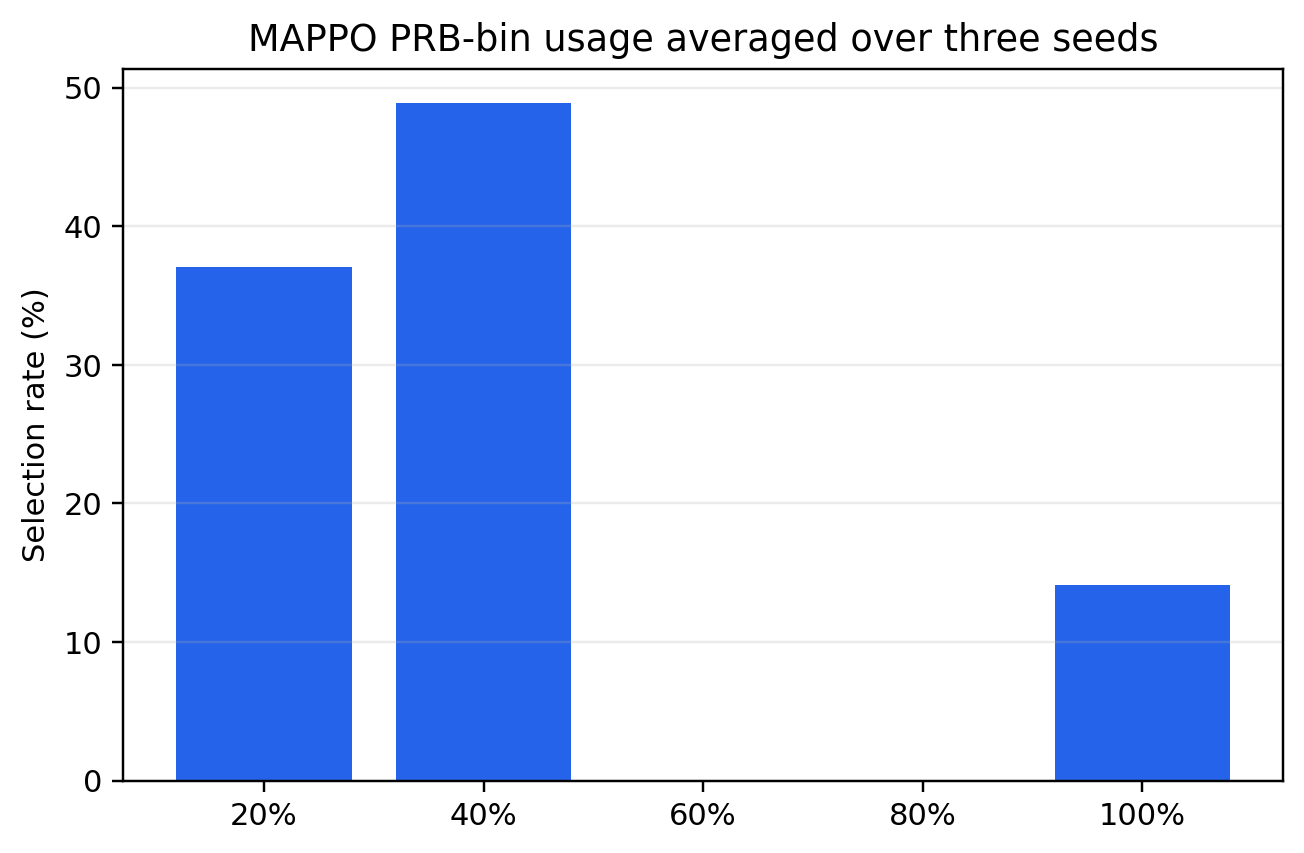
\includegraphics[width=0.82\textwidth]{figures/mappo_prb_distribution.png}
    \caption{MAPPO PRB-bin selection distribution averaged over three seeds.}
    \label{fig:mappo-prb-distribution}
\end{figure}

This behavior indicates that the policy has learned a conservative bandwidth-allocation strategy. Most tasks receive a moderate reservation rather than a maximum one, which helps preserve PRBs for other devices while still maintaining high task success. The occasional use of the \(100\%\) bin suggests that the policy escalates bandwidth only for harder communication conditions or more urgent tasks.

\subsection{Ablation and PPO Baseline Discussion}
\label{subsec:ablation-discussion}

A full ablation suite is not yet preserved as structured output in the current workspace, so this report does not claim a complete numerical decomposition of every model component. Nevertheless, the available PPO comparison provides two useful observations.

First, on-policy learning itself is effective in this environment: both PPO and MAPPO improve steeply during early training. Second, MAPPO is the more complete and reliable artifact in the present repository, and it is the one that achieves the robust three-seed evaluation reported above. Since the key architectural difference is the addition of agent embeddings and a centralized critic tied to the MARL formulation, the available evidence supports the conclusion that explicit multi-agent modeling is beneficial for this task.

The current artifact does not yet provide a separate controlled run with the PRB head removed. That study remains a useful next step because the PRB distribution in \Figref{fig:mappo-prb-distribution} strongly suggests that bandwidth decisions are an active component of the learned policy rather than a redundant output head.

\subsection{Robustness Across Random Seeds}
\label{subsec:robustness}

The multi-seed MAPPO evaluation is summarized in \Tabref{tab:mappo-robustness}. The standard deviation of task success is below \(0.01\%\), and the total-time and energy variations are also modest. Such consistency is important because it shows that the learned policy is not an artifact of one favorable random seed.

\begin{table}[htbp]
    \centering
    \begin{tabular}{p{0.20\linewidth}ccc}
        \hline
        \textbf{Seed} & \textbf{Success rate (\%)} & \textbf{Avg total time (s)} & \textbf{Energy} \\
        \hline
        9001 & 99.9346 & 4.5587 & 231.0655 \\
        9002 & 99.9346 & 4.5175 & 219.7854 \\
        9003 & 99.9510 & 4.5540 & 227.3956 \\
        Mean & 99.9401 & 4.5434 & 226.0822 \\
        Std. dev. & 0.0077 & 0.0184 & 4.6998 \\
        \hline
    \end{tabular}
    \caption{MAPPO robustness under three independent evaluation seeds.}
    \label{tab:mappo-robustness}
\end{table}

\subsection{Summary}
\label{subsec:results-summary}

The experimental evidence supports three main conclusions. First, MAPPO learns quickly and reaches a near-saturated task success rate within a relatively short training budget. Second, the learned policy achieves a stronger latency-success trade-off than the representative heuristic baselines preserved in the current artifact. Third, the destination and PRB distributions show that the policy is using the full three-tier architecture and the wireless resource allocator in a non-trivial way.

The main remaining gap is not methodological but experimental packaging: some heuristic baseline results are preserved as dashboards rather than structured tables. Once those baselines are rerun with consistent CSV export, the report can be extended with a full all-algorithm comparison table without changing the rest of the methodology.
